\documentclass[class=report,crop=false, 12pt]{standalone}
\usepackage{../scratch}


\begin{document}


\titre{Projet -- Scratch et informatique au collège}
%=========================


\pagestyle{empty}

\section{Objectifs}

Les objectifs principaux sont :
\begin{enumerate}
\item initiation à l'informatique,
\item initiation au codage.
\end{enumerate}


Ce cours est destiné dans un premier temps aux enseignants de mathématiques, qui vont enseigner l'informatique à travers le nouveau programme 2016.
Cependant les ressources produites sont directement exploitables en classes.


\section{Scratch}

Commençons par le langage choisi.

\begin{minipage}{0.7\textwidth}
\begin{itemize}
  \item Scratch est un langage de programmation pour débutants. 
  \item Les instructions sont des blocs à déplacer.
  \item Le programmation est donc visuelle, sans erreurs de syntaxe possibles.
  \item Scratch est largement diffusé et utilisé dans le monde entier.
  \item Il existe déjà de nombreux projets, qu'il est possible de réutiliser.
\end{itemize}
\end{minipage}
\begin{minipage}{0.29\textwidth}
  \centering
  
\includegraphics[width = 4cm]{Scratchcat}
\end{minipage}



\section{Initiation au codage}

\`A la fin du cours les élèves doivent :
\begin{itemize}
  \item savoir déplacer le lutin,

  \item savoir coder des petits programmes,
    
  \item utiliser des boucles, des tests,
  
  \item analyser un programme, trouver les erreurs, les corriger.
\end{itemize}

\begin{center}
  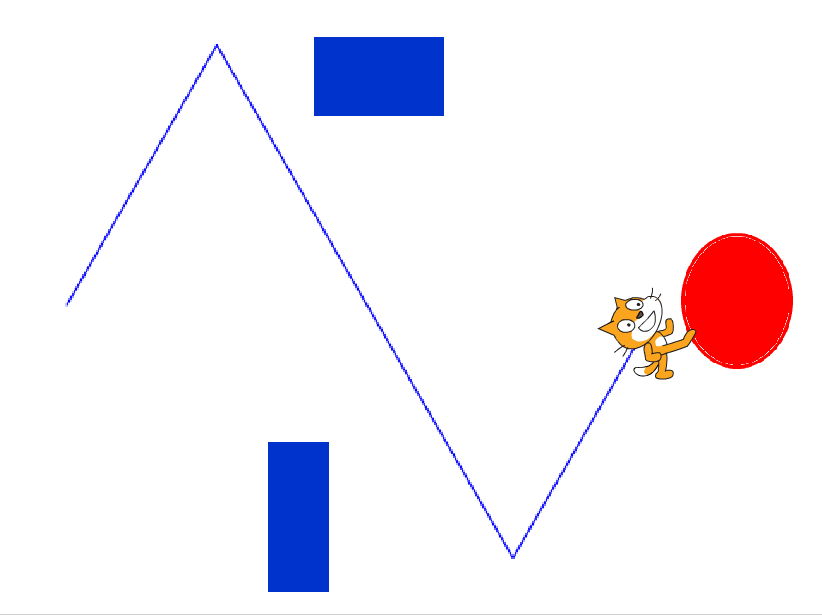
\includegraphics[width=0.5\textwidth]{../fiche04/ecran-04-ex1} 
\end{center}

\section{Initiation à l'informatique}

Le but est de découvrir plusieurs notions théoriques d'informatique à travers des activités ludiques, numériques, graphiques...
Ces activités sont des activités débranchées, sur feuille. 

Il y a bien sûr, un aspect très pragmatique : le jour où les ordinateurs refusent de démarrer, on peut quand même faire une séance d'informatique.

Mais une activité sur feuille, permet surtout de :
\begin{itemize}
  \item préparer à des notions générales (déplacement, repères,...) pour ensuite passer sereinement et efficacement à une séance pratique, 
  
  \item comprendre des notions importantes, indépendamment du langage choisi (boucles, test, vrai \slash faux,...),
  
  \item réfléchir à l'écriture du programme avant de le coder,
  
  \item aborder des notions plus difficiles, plus théoriques, ou pas adaptées à Scratch (binaire, cryptographie, base de données,...),
  
  \item faire des activités graphiques (couleurs, triangulation, pixels,...)
\end{itemize}

\myfigure{1}{
\tikzinput{../pixels/pixels-ex2-01}
}

\section{Méthode}

\begin{itemize}
\item Le niveau est collège (cycle 4: 5ème, 4ème, 3ème).
\item Le travail est découpé en séances.
\item Chaque séance représente au moins 3h de travail :
  \begin{itemize}
    \item une heure de travail sur feuille, avec des activités non liées à
  Scratch, mais qui préparent le travail sur Scratch,
    \item une heure de travail dirigé sur machine, avec des activités sur
  Scratch, corrigées en vidéo,
    \item une heure pour résoudre des énigmes en autonomie.
  \end{itemize}
\end{itemize}

\bigskip
\bigskip

Notre approche se distingue des autres par :
\begin{itemize}
  \item des ressources entièrement gratuites, réutilisables et modifiables,
  \item une approche qui n'est pas uniquement ludique, mais aussi plus théorique et plus scolaire, donc adaptée à l'enseignement en classes,
  \item un réinvestissement des notions mathématiques (repère, angles, calcul algébrique) qui permet au professeur de mathématique de faire le lien math/info.
\end{itemize}


\section{Productions}

\begin{itemize}
  \item Une vingtaine de fiches de travail sur feuilles : travail bien avancé, déjà 100 pages A4.

  \item Une quinzaine de fiche d'activités Scratch (3 activités par fiches) : sur feuille et en vidéo. 
  Environ la moitié des fiches sont prêtes, une série de vidéos tests a été tournée. Les vraies vidéos seront enregistrées en fin de projet.
  
  \item Une quinzaine de fiche d'énigmes (3 énigmes par fiches) : afin d'évaluer les apprentissages. Environ la moitié des fiches sont prêtes.
  
  \item En fin de projet, il y aurait donc un livre (environ 250 pages) et environ 50 vidéos.
  
  \item Un MOOC serait donné pour diffuser tout le travail.
\end{itemize}

\section{Personnes}

Ce projet est porté par des personnes de l'université de Lille, avec le concours de l'IREM  (institut de recherche sur l'enseignement des mathématiques) et du groupe de travail "Numérique au collège" constitué d'enseignants de mathématiques en collège.

\bigskip

Contact :
\begin{itemize}
  \item Arnaud Bodin (université Lille 1) \href{mailto:Arnaud.Bodin@math.univ-lille1.fr}{Arnaud.Bodin@math.univ-lille1.fr}
  
  \item François Recher (université Lille 1, IREM de Lille) \href{mailto:Francois.Rechern@math.univ-lille1.fr}{François.Recher@math.univ-lille1.fr}
\end{itemize}


\section{Besoin}

Le budget total estimé du projet est $10\, 000$ euros, afin de financer :
\begin{itemize}
  \item la réalisation et le montage des vidéos,
  \item des heures de décharge pour les enseignants-chercheurs (écriture, vidéo, MOOC,...)
  \item des heures de vacations pour les enseignants du second degré (écriture, tests grandeur nature,...),
  \item l'achat de matériel informatique,
  \item l'achat d'exemplaires du livre produit.
\end{itemize}


\end{document}

